\documentclass[a4paper]{article}
\usepackage[utf8]{inputenc}
\usepackage{amsmath}
\usepackage{siunitx}
\usepackage[ngerman]{babel}
\usepackage{pgfplots}
\usepackage{hyperref}
\usepackage{pgfplotstable}
\usepackage[section]{placeins}
\usepackage{enumitem}
\usepackage{float}

\pgfplotsset{compat=1.15}

\title{GPET\\ Auswertung Versuch 4\\ Gruppe 1}

\author{Jonas Otto\\ \href{mailto:jonas@jonasotto.com}{jonas@jonasotto.com} 
   \and Luca Krüger \\ \href{mailto:luca.krueger@uni-ulm.de}{luca.krueger@uni-ulm.de} }
\date{8. Mai 2018}

\begin{document}
    
\maketitle

\section{Versuchsauswertung}

\subsection{Ein- und Ausschaltvorgang einer Induktivität}
\begin{figure}[H]
    \centering
    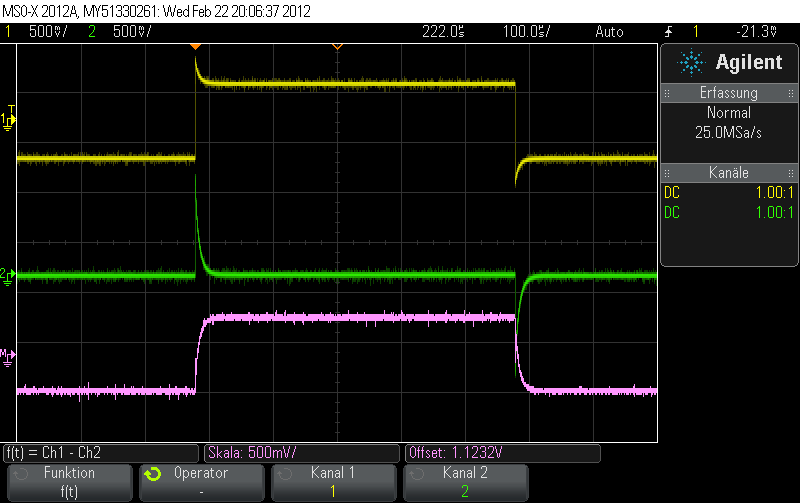
\includegraphics[width=0.8\textwidth]{versuch1_1.png}
    \caption{Eingangsspannung (gelb), Spannung an der Spule (grün), Differenzspannung($\sim$ Strom)(rosa) }
    \label{fig:versuch1-1}
\end{figure}
In diesem Versuch wurden Ein- und Ausschaltvorgänge untersucht. Ausschaltvorgänge verhalten sich äquivalent zu Einschaltvorgängen. im folgenden wird deshalb exemplarisch ein Einschaltvorgang betrachtet.
Das Einschalten wurde mithilfe des internen Funktionsgenerators des Oszilloskops bei simuliert.
In Abbildung \ref{fig:versuch1-1} ist der Einschaltvorgang einer Induktivität zu sehen. Der grüne Graph ist der Spannungsverlauf an der Induktivität. Der Ausgang vom Frequenzgenerator wurde über Kanal$1$ gemessen und im gelben Graph dargestellt. Es fällt auf, dass die Schaltung den Ausgang des Frequenzgenerators leicht beeinflusst. Dies bei folgenden Betrachtungen zu vernachlässigen. 
Der rosafarbene Graph stellt die Differenz aus beiden Spannungsverläufen dar, also die Spannung, die über dem Widerstand abfällt. Durch $I=\frac{U}{R}$ ist der Spannungsverlauf proportional zum Strom in der Schaltung, also auch zum Strom durch die Induktivität.
Die Spannung über der Induktivität fällt nach dem Einschalten schnell ab, der Strom steigt an. Dieses Verhalten deckt sich mit dem Einschaltvorgang an einer Induktivität, wie es in der Vorlesung GET$1$ behandelt wurde.
\subsection{Freie Schwingungen}
\paragraph{1.}
\begin{figure}[H]
    \centering
    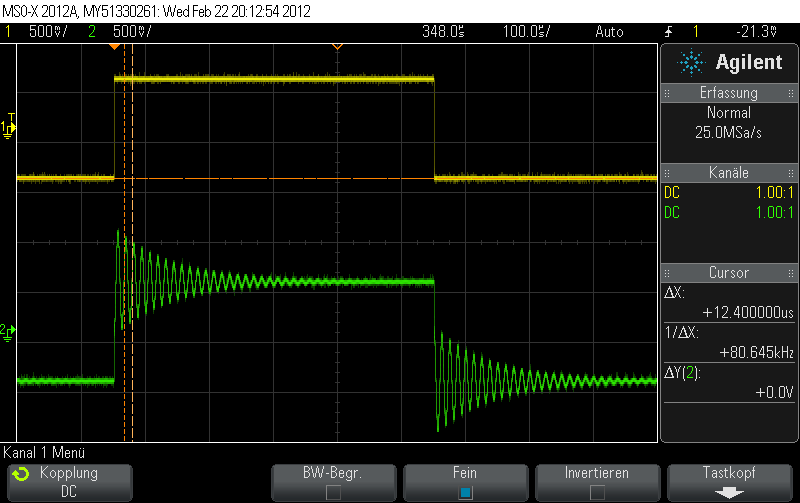
\includegraphics[width=0.8\textwidth]{versuch2_1.png}
    \caption{Eingangsspannung, Spannung $U_1$ an der Induktivität gemessen}
    \label{fig:versuch2-1}
\end{figure}

\begin{figure}[H]
    \centering
    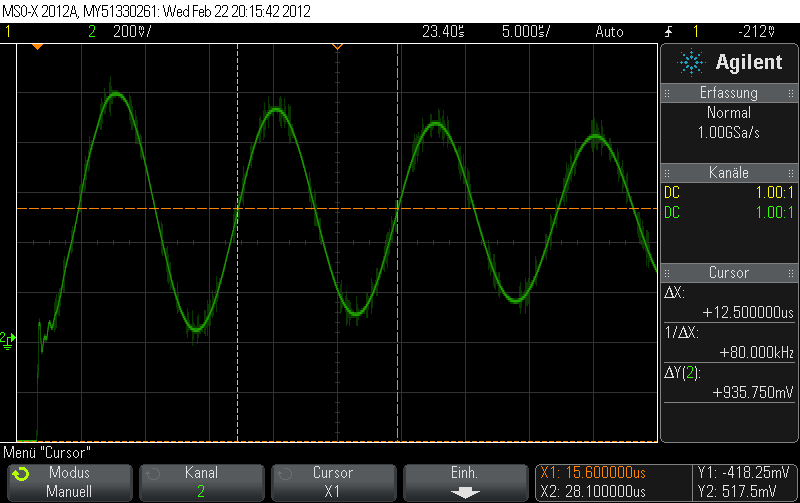
\includegraphics[width=0.8\textwidth]{versuch2_1_frequenz.png}
    \caption{Eingangsspannung, Spannung $U_1$ an der Induktivität gemessen}
    \label{fig:versuch2-1-frequenz}
\end{figure}

Wie in Abbildung \ref{fig:versuch2-1-frequenz} ersichtlich, beträgt die Frequenz $f=\frac{1}{T}=\frac{1}{12.5\si{\micro s}}=80\si{kHz}$.
Die Kapazität berechnet sich durch $f_0=\frac{1}{2\pi\sqrt{LC}}\Leftrightarrow C=\frac{1}{f^24\pi^2L}\approx 220\si{pF}$

\begin{figure}[H]
    \centering
    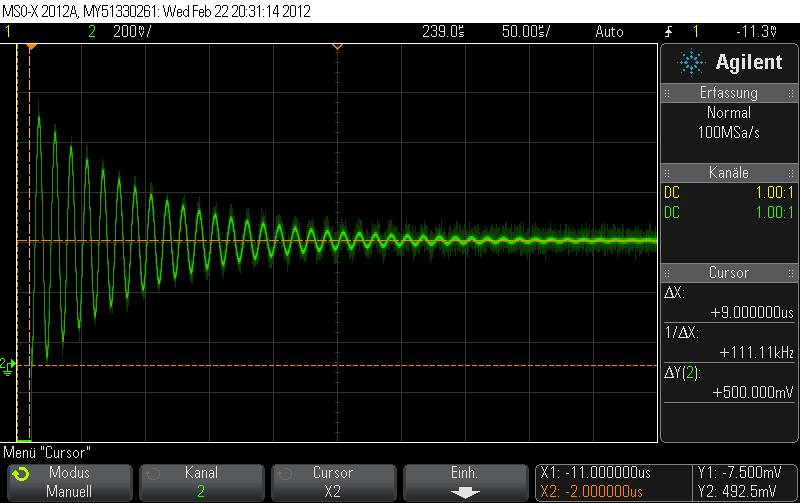
\includegraphics[width=0.8\textwidth]{versuch2_1_amplitude.png}
    \caption{Eingangsspannung, Spannung $U_1$ an der Induktivität gemessen}
    \label{fig:versuch2-1-amplitude}
\end{figure}

In Abbildung \ref{fig:versuch2-1-amplitude} ist die Amplitude der auftretenden Eigenschwingung zu sehen. Anfangs  beträgt sie $\approx 500\si{mV}$, fällt dann aber schnell ab.

\paragraph{2.}
In diesem Versuch wird zur Induktivität eine Kapazität in Reihe geschaltet und dann die Spannung an der Kapazität gemessen. Die Rechteckspannung am Eingang hat nach wie vor eine Frequenz von $10\si{kHz}$.
In Abbildung \ref{fig:versuch2-2-frequenz} wird ersichtlich, dass die Frequenz $f=\frac{1}{T}=\frac{1}{258\si{\micro s}}=3.88\si{kHz}$ beträgt. In Abbildung \ref{fig:versuch2-2-amplitude} wurde die Abnahme der Amplitude gemessen, die $237.5\si{mV}$ von der ersten zur zweiten Spitze beträgt.

\begin{figure}[H]
    \centering
    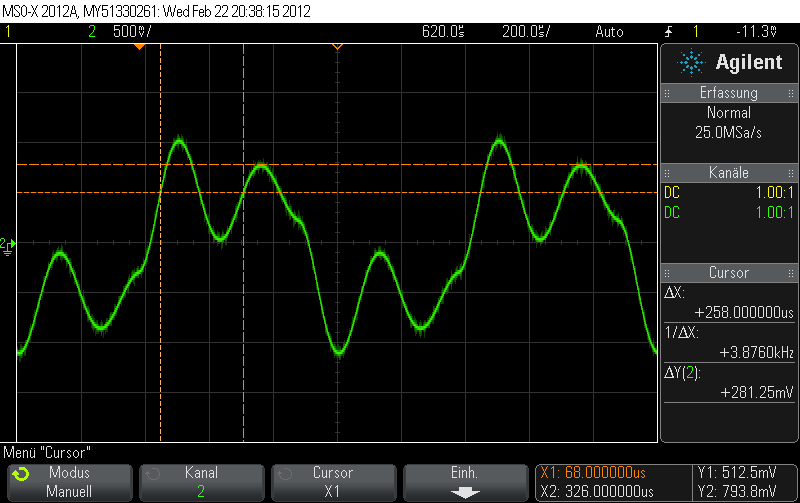
\includegraphics[width=0.8\textwidth]{versuch2_2_frequenz.png}
    \caption{Frequenz von $U_1$ am Kondensator}
    \label{fig:versuch2-2-frequenz}
\end{figure}


\begin{figure}[H]
    \centering
    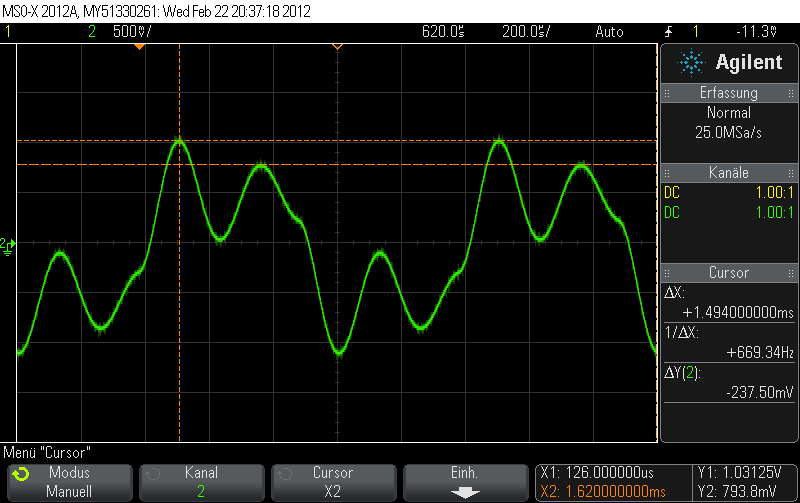
\includegraphics[width=0.8\textwidth]{versuch2_2_amplitude.png}
    \caption{Amplitudenabnahme von $U_1$ am Kondensator}
    \label{fig:versuch2-2-amplitude}
\end{figure}


\paragraph{3.}
Hier wird dem vorherigen Versuch noch ein Potentiometer in Reihe geschaltet, welches auf verschiedene Werte zwischen $0\si{\ohm}$ und $800\si{\ohm}$ eingestellt wird.
In Abbildung \ref{fig:versuch2-3-100ohm} ist der Spannungverlauf bei $R=100\si{\ohm}$ zu sehen, Abbildung \ref{fig:versuch2-3-400ohm} zeigt die Spannung bei $R=400\si{\ohm}$, Abbildung \ref{fig:versuch2-3-700ohm} bei $700\si{\ohm}$. Allgemein ist zu erkennen, dass bei höherem Widerstand die Schwingung stärker gedämpft wird.

\begin{figure}[H]
    \centering
    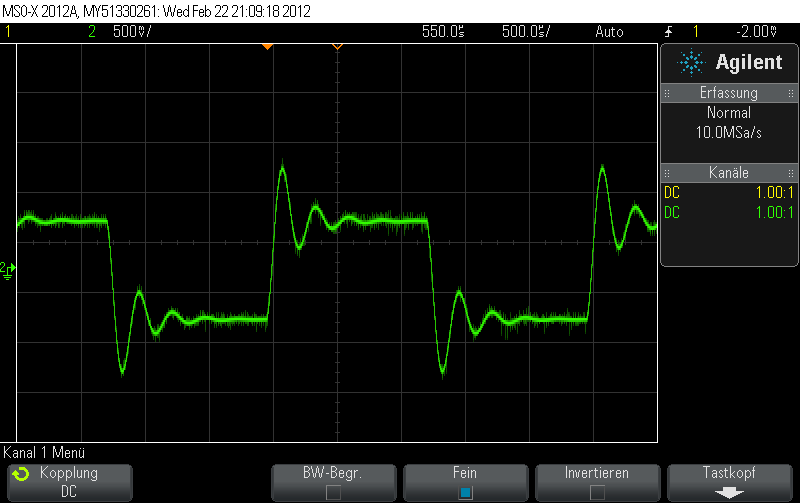
\includegraphics[width=0.8\textwidth]{versuch2_3_100ohm.png}
    \caption{Spannung $U_1$ über Kapazität und $R=100\si{\ohm}$}
    \label{fig:versuch2-3-100ohm}
\end{figure}

\begin{figure}[H]
    \centering
    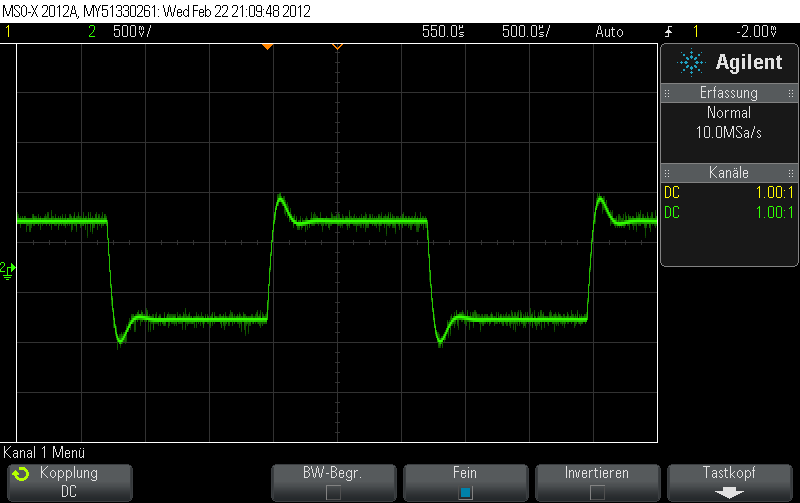
\includegraphics[width=0.8\textwidth]{versuch2_3_400ohm.png}
    \caption{Spannung $U_1$ über Kapazität und $R=400\si{\ohm}$}
    \label{fig:versuch2-3-400ohm}
\end{figure}

\begin{figure}[H]
    \centering
    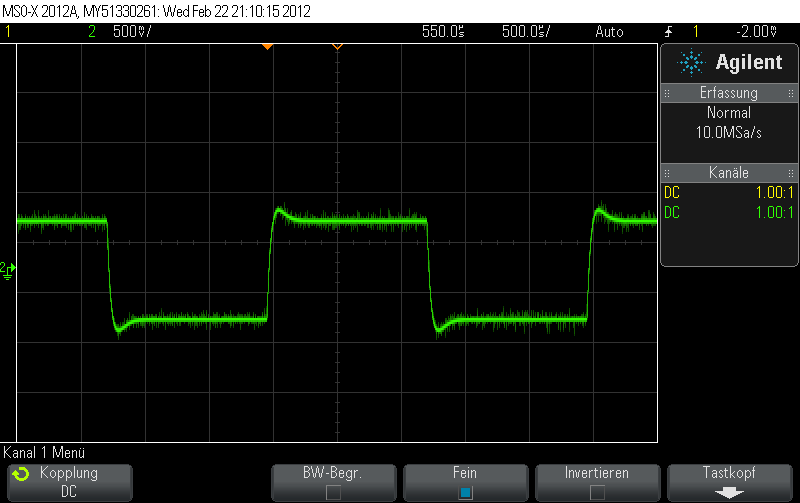
\includegraphics[width=0.8\textwidth]{versuch2_3_700ohm.png}
    \caption{Spannung $U_1$ über Kapazität und $R=700\si{\ohm}$}
    \label{fig:versuch2-3-700ohm}
\end{figure}

Abbildung \ref{fig:versuch2-3-15ohm-frequenz} zeigt die Spannung bei $R=15\si{\ohm}$.
Mittels Cursor am Oszilloskop wurde eine Frequenz von $f=\frac{1}{T}=\frac{1}{254\si{\micro s}}=3.9\si{kHz}$ und eine Amplitudenabnahme von $332.5\si{mV}$ vom ersten zum zweiten Peak ermittelt (Abbildung \ref{fig:versuch2-3-15ohm-frequenz} und \ref{fig:versuch2-3-15ohm-amplitude}).

\begin{figure}[H]
    \centering
    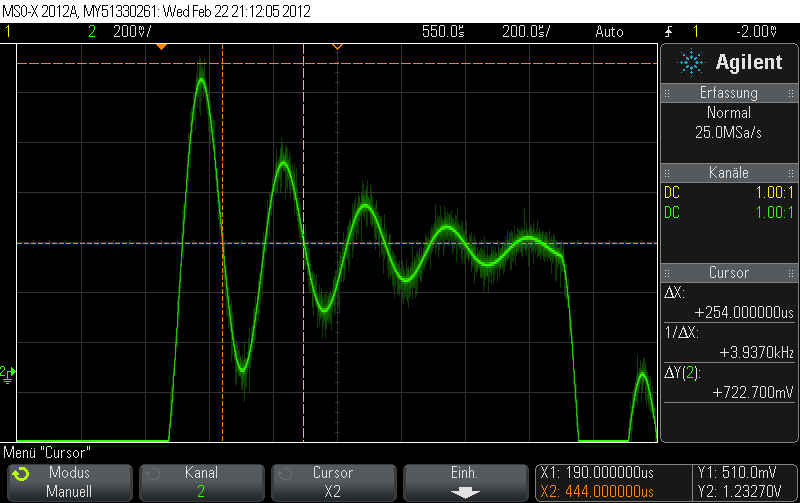
\includegraphics[width=0.8\textwidth]{versuch2_3_15ohm_frequenz.png}
    \caption{Messung der Frequenz bei $R=15\si{\ohm}$}
    \label{fig:versuch2-3-15ohm-frequenz}
\end{figure}

\begin{figure}[H]
    \centering
    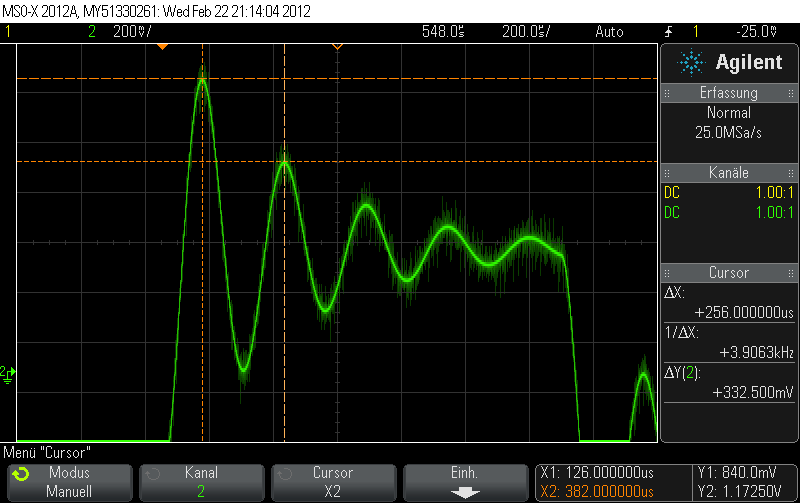
\includegraphics[width=0.8\textwidth]{versuch2_3_15ohm_amplitude.png}
    \caption{Messung der Amplitudenabnahme bei $R=15\si{\ohm}$}
    \label{fig:versuch2-3-15ohm-amplitude}
\end{figure}

\subsection{Spannungsüberhöhung}
In diesem Versuch wird die Spannungserhöhung in einem L-C-Reihenschwingkreis untersucht.
\paragraph{1.}
Ein Maximum der Spannung $U_2$ am Kondensator wird erwartet, wenn die Resonanzfrequenz angelegt wird.
Diese berechnet sich durch $f_0=\frac{1}{2\pi\sqrt{LC}}=3751\si{Hz}$
Dies bestätigt sich auch im Frequenz-Sweep (Abbildung \ref{fig:versuch3-sweep}), der eine hohe Amplitude sehr nahe der berechneten Frequenz zeigt.

\begin{figure}[H]
    \centering
    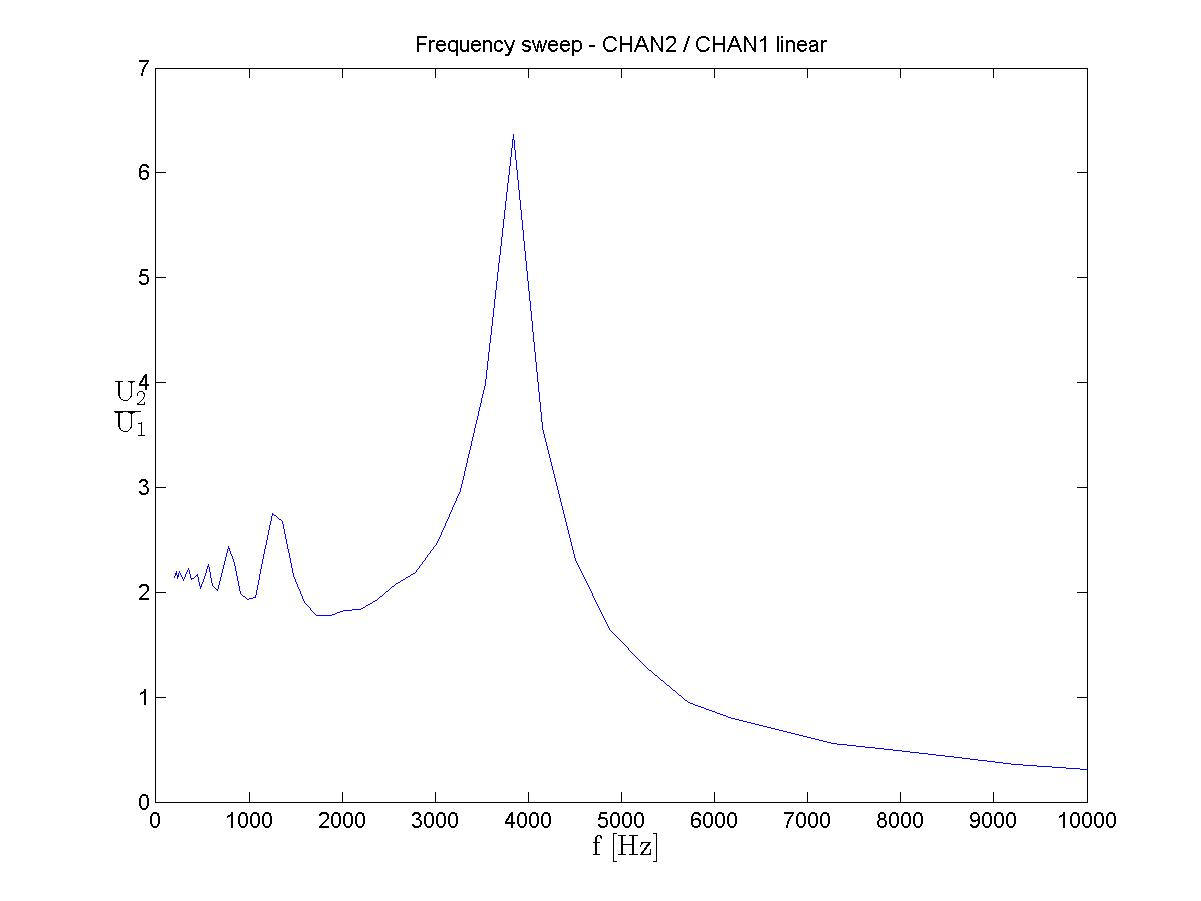
\includegraphics[width=0.8\textwidth]{versuch3_sweep_ylinxlin1.jpg}
    \caption{Frequenz Sweep über Reihenschwingkreis}
    \label{fig:versuch3-sweep}
\end{figure}

\subsection{Induktionsschleife einer Ampelschaltung}
\paragraph{1.}
Bei Resonanzfrequenz ist zu erkennen, dass die Amplitude maximal ist (Abbildung \ref{fig:versuch4-resonanz}). Die Amplitude beträgt hier $3.2125\si{V}$, die Frequenz $3.76\si{kHz}$.

\begin{figure}[H]
    \centering
    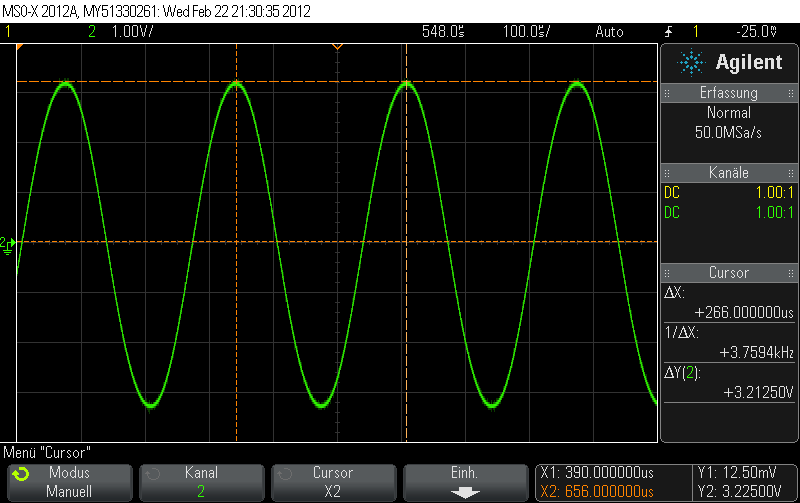
\includegraphics[width=0.8\textwidth]{versuch4_maxamplitude.png}
    \caption{L-C-Reihenschwingkreis bei Resonanzfrequenz}
    \label{fig:versuch4-resonanz}
\end{figure}

\paragraph{2.}
In diesem Versuch wird ein Eisenkern in die Spule eingeführt und der Spannungsverlauf beobachtet.
Wenn ein Eisenkern in die Spule eingeführt wird, ist zu erkennen, dass die Amplitude nicht mehr maximal ist. Dies liegt daran, dass der Eisenkern die Induktivität und damit Impedanz der Spule verändert, sodass die angelegte Frequenz nicht mehr der Resonanzfrequenz entspricht. In Abbildung \ref{fig:versuch4-minamplitude} ist zu erkennen, dass die Amplitude nun deutlich unter der bei Resonanz liegt.

\begin{figure}[H]
    \centering
    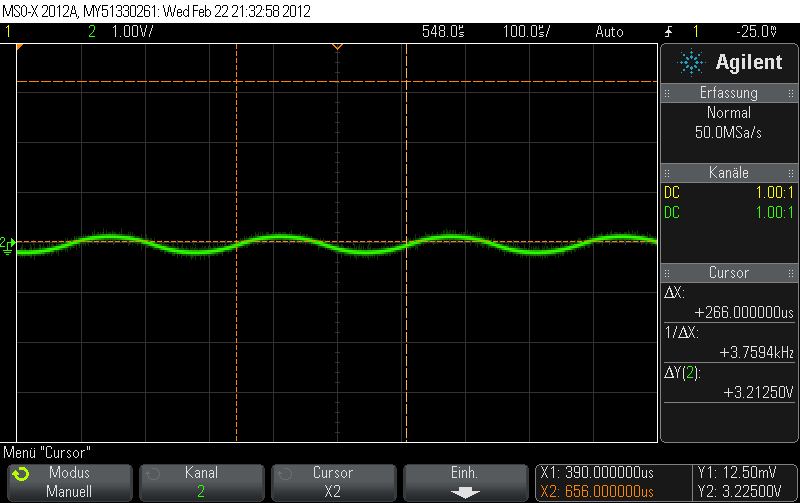
\includegraphics[width=0.8\textwidth]{versuch4_lowamplitude.png}
    \caption{L-C-Reihenschwingkreis mit Eisenkern}
    \label{fig:versuch4-minamplitude}
\end{figure}

\paragraph{3.}
Wenn wiederholt ein Frequenz-Sweep durchgeführt wird (Abbildung \ref{fig:versuch4-eisenkern-sweep}), ist ersichtlich, dass sich die Resonanzfrequenz verschoben hat. Diese liegt nun bei etwas unter $2000\si{Hz}$.

\begin{figure}[H]
    \centering
    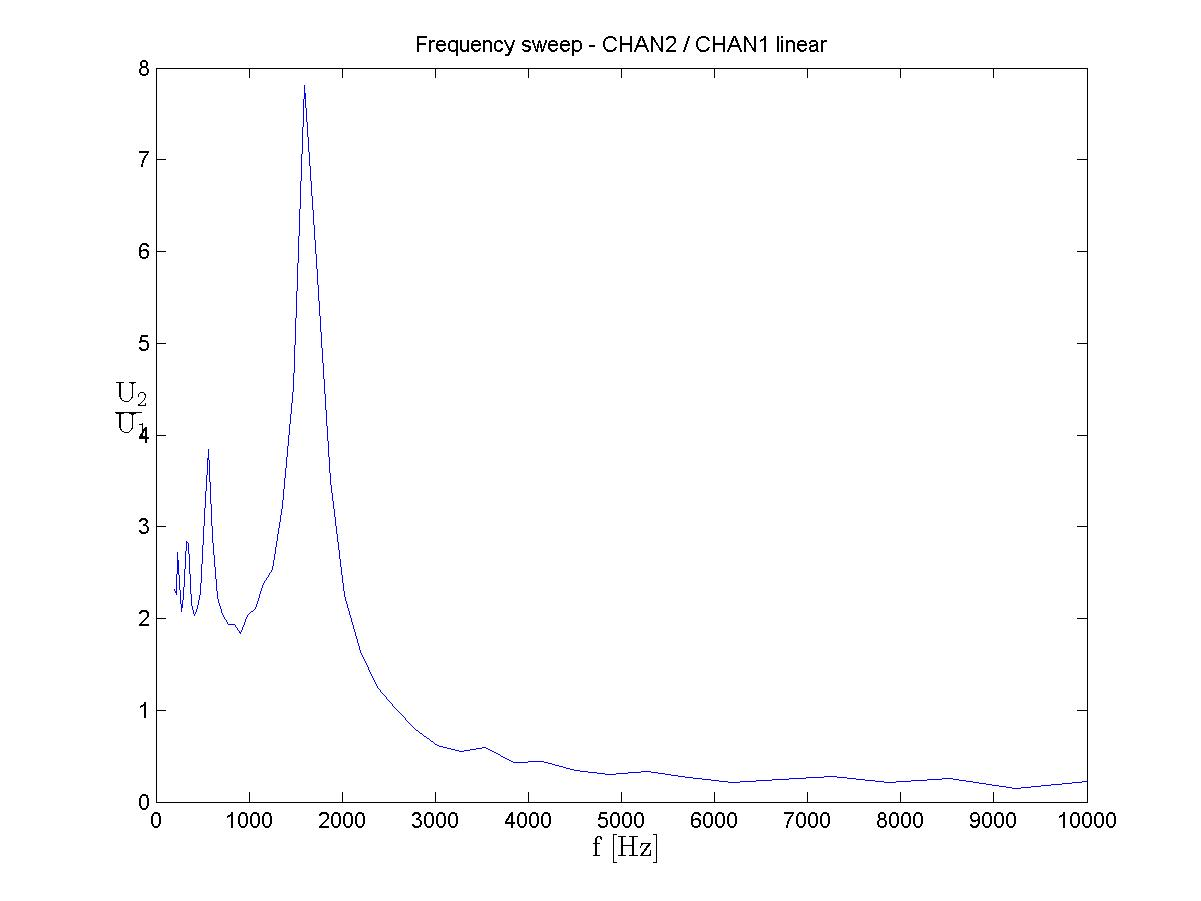
\includegraphics[width=0.8\textwidth]{versuch4_eisenkern_sweep_ylinxlin.jpg}
    \caption{Frequenz-Sweep L-C-Reihenschwingkreis mit Eisenkern}
    \label{fig:versuch4-eisenkern-sweep}
\end{figure}

\subsection{Analyse einer unbekannten Schaltung}
\paragraph{1.}
Zur Analyse der unbekannten Schaltung wird ein Frequenz-Sweep von $1\si{Hz}$ bis $250\si{kHz}$ durchgeführt (Abbildung \ref{fig:versuch5-sweep}). Das Verhalten entspricht dem einer Bandsperre.
Das bedeutet, dass es sich um einen Reihenschwingkreis handelt, bei dem die Impedanz bei Resonanzfrequenz gegen 0 geht. Dies entspricht Schaltung A, da das Verhalten bei $f=0, f=f_0, f=\infty$ übereinstimmt (Siehe 2.).

\begin{figure}[H]
    \centering
    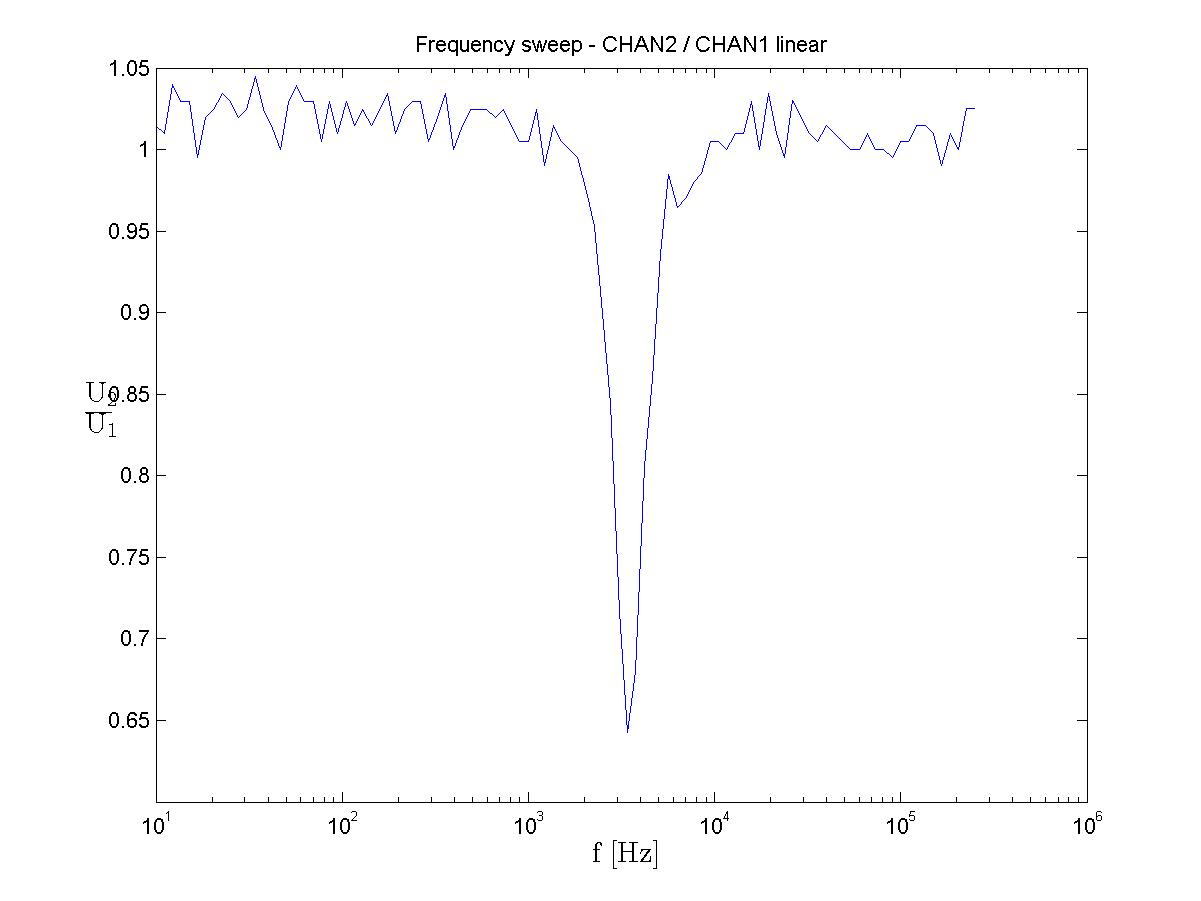
\includegraphics[width=0.8\textwidth]{versuch5_sweep_ylinxlog.jpg}
    \caption{Frequenz-Sweep der unbekannten Schaltung}
    \label{fig:versuch5-sweep}
\end{figure}

\paragraph{2.}

\begin{itemize}
    \item{A: 
        \begin{itemize}
            \item $f=0\si{Hz}$: Kondensator sperrt, $\frac{U_2}{U_1} = 1$
            \item $f=f_0$: $Z=Z_R$
            \item $f=\infty$: Spule sperrt, $\frac{U_2}{U_1} = 1$
        \end{itemize}
    }
    
    \item{B: 
        \begin{itemize}
            \item $f=0\si{Hz}$: Kondensator sperrt, $\frac{U_2}{U_1} = 1$
            \item $f=f_0$: Reihenschwingkreis leitet, $Z=0$
            \item $f=\infty$: Spule sperrt, Kondensator leitet, $\frac{U_2}{U_1} = \frac{R_{innen}}{R_1}$ (Hier: $\frac{U_2}{U_1} = 1$)
        \end{itemize}
    }
    
    \item{C: 
        \begin{itemize}
            \item $f=0\si{Hz}$: $Z=R$, da Spule leitet
            \item $f=f_0$: Parallelschwingkreis sperrt, $\frac{U_2}{U_1} = 1$ (Hier:$Z=R$, $\frac{U_2}{U_1} = \frac{R_{innen}}{R_1}$)
            \item $f=\infty$:  $Z=R$, da Kondensator nicht leitet
        \end{itemize}
    }
    
    \item{D: 
        \begin{itemize}
            \item $f=0\si{Hz}$: $Z=R$ (Hier: $Z=\infty$)
            \item $f=f_0$: Reihenschwingkreis leitet, $Z=0$
            \item $f=\infty$: Spule sperrt, $Z=\infty$
        \end{itemize}
    }
    
    \item{E: 
        \begin{itemize}
            \item $f=0\si{Hz}$: $Z=0$ (Hier: $Z=\infty$)
            \item $f=f_0$: $Z=R$
            \item $f=\infty$: $Z=0$
        \end{itemize}
    }
    
\end{itemize}
\end{document}